\section{什么是计算机科学}

\begin{frame}\ft{\secname}
  所谓计算机科学,即
  \begin{itemize}
  \item 研究问题
  \item 解决问题
  \item 生成解决问题的方案
  \end{itemize}
  给定一个问题,目标是开发算法,编写程序,用于解决可能出现的问题。%算法遵循它有限的过程就可以解决问题。
\end{frame}

% \begin{frame}\ft{\secname}
% 计算机科学可以被认为是对算法的研究。但是,我们必须清楚地认识到,一些问题可能没有解决方案。虽然证明这种说法正确性超出了本文的范围,但一些问题不能解决的事实对于那些研究计算机科学的人是很重要的。可以这么说,计算机科学研究有解决方案和没有解决方案的问题。
% \end{frame}

% \begin{frame}\ft{\secname}
% 当描述问题及其解决方案时,会提到计算一词。若存在一个算法解决某个问题,就称该问题是可计算的。计算机科学的另一个定义是:计算机科学是研究那些可计算和不可计算的问题,研究是不是存在一种算法来解决它。请注意这里没有涉及到“计算机”一词,解决方案与机器无关。
% \end{frame}

\begin{frame}\ft{\secname}
计算机科学,因涉及问题解决过程本身,是关于抽象的研究。抽象使我们能从逻辑视角和物理视角来分别看待问题及其解决方案。%基本思想跟我们常见的例子一样。
\end{frame}

\begin{frame}\ft{\secname}
  \begin{figure}
  	\centering
  	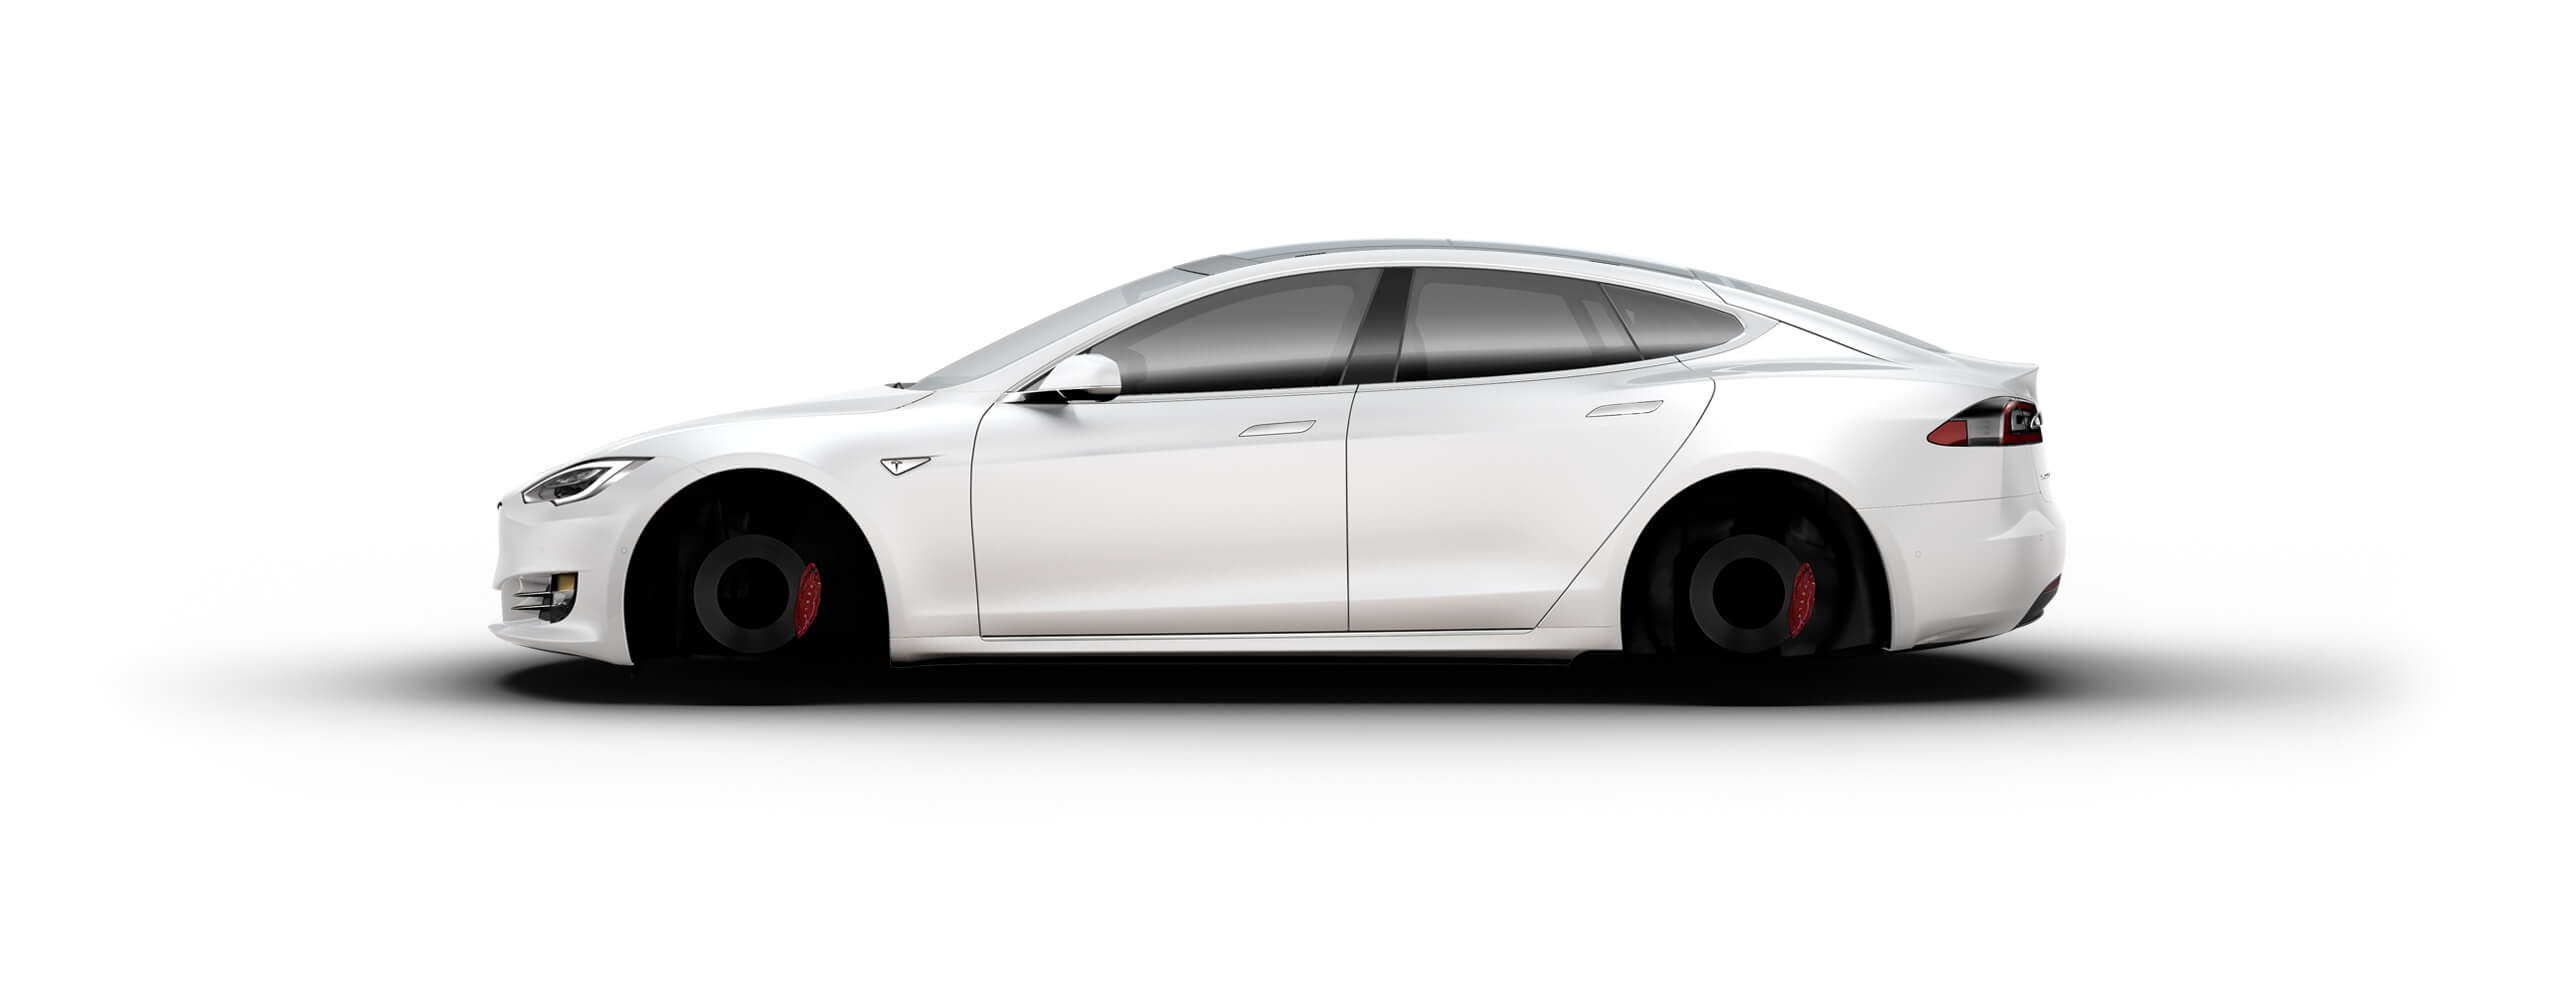
\includegraphics[width=3.5in]{images/car.jpg}
  \end{figure} \pause 
  \begin{itemize}
  \item   作为司机,你会与车有一些互动,如上车、插钥匙、点火、换挡、制动、加速、转向、下车等。你只需要了解车一些基本功能,就可以操纵它。\\
  \item[] 此时,你所看到的是汽车的“逻辑视角”,这些功能通常称为“接口”。 \\[0.1in] \pause 
  
  \item   作为修车师傅,看待汽车的视角就会截然不同。你不仅需要知道如何开车,还必须知道汽车的一些内部细节,比如说发动机如何工作、变速箱如何变速、温度如何控制等等。
  \item[] 这就是“物理视角”,细节发生在“引擎盖下”。
    
  \end{itemize}
\end{frame}

\begin{frame}\ft{\secname}
  \begin{figure}
  	\centering
  	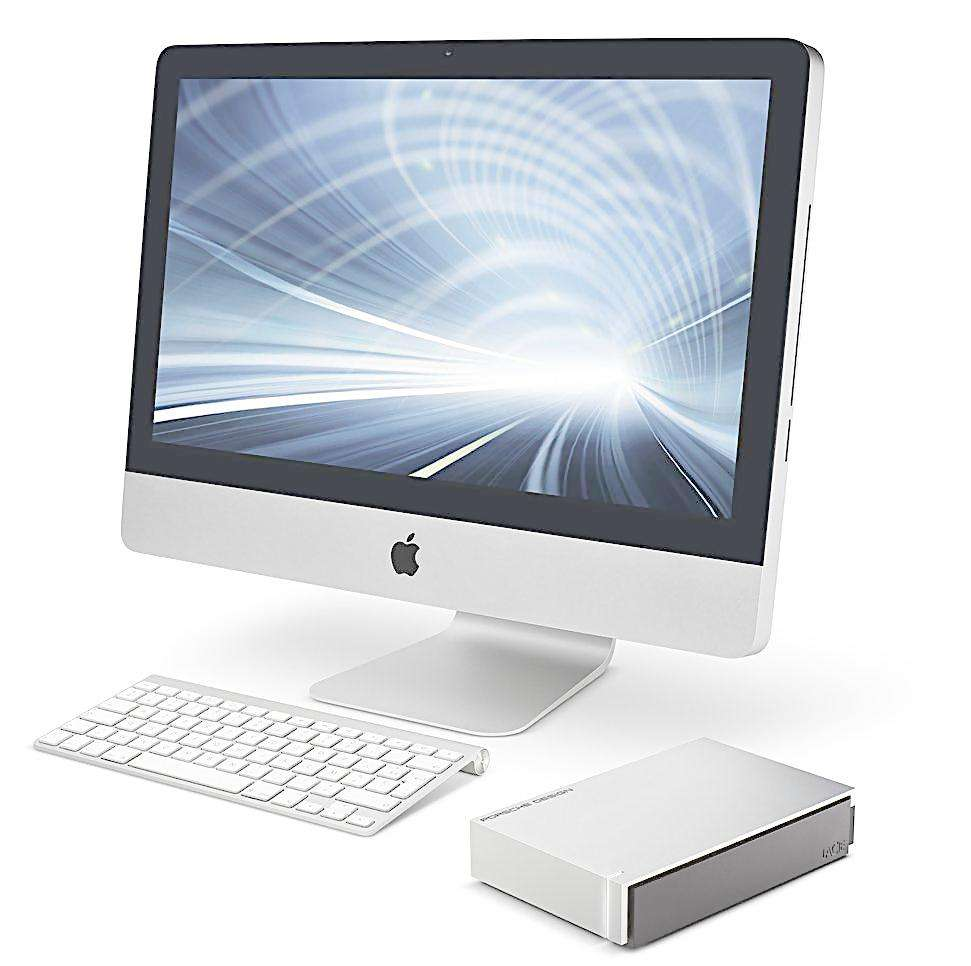
\includegraphics[width=1.5in]{images/computer.jpeg}
  \end{figure} \pause 
  \begin{itemize}
  \item 作为用户,你可以编写文档、收发邮件、上网冲浪、播放音乐、存储图像和玩游戏等,但你并不知道这些APP工作的细节。
  \item[] 此时,你是从逻辑或用户角度看待计算机。 \\[0.1in] \pause 
  \item 作为计算机科学家、程序员、技术支持人员和系统管理员,你看待计算机的角度会截然不同。你必须知道操作系统如何工作、如何配置网络协议、如何编写控制功能的各种脚本。
  \item[] 总之,你必须能够控制底层的细节。

  \end{itemize}

\end{frame}

\begin{frame}[fragile]\ft{\secname}

  作为用户,你不需要知道细节,只需了解接口的工作方式。接口是用户与底层沟通的窗口。

\end{frame}

\begin{frame}[fragile]\ft{\secname}

  看一个抽象的例子---Python 数学模块。一旦导入模块,就可以执行计算
\begin{lstlisting}
  >>> import math
  >>> math.sqrt(16)
  4.0
\end{lstlisting} \pause 

你无需知道计算平方根的细节,只需知道sqrt函数的功能及其使用方式。这就像一个“黑盒子”,其接口可描述为:函数名、参数、返回值,其细节隐藏在内部。
\begin{figure}[htbp]
  \centering
  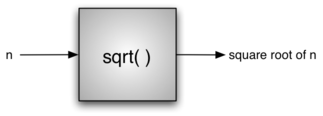
\includegraphics[width=2in]{images/blackbox.png}
\end{figure}

\end{frame}

